\chapter{Introduction}
\section{Context}
\subsection{3D viewers}
-> Applications?

-> Who uses them?

-> What for?

\subsection{\acs{bim} geometry} \label{subsec:bimGeometry}
% -> What is \ac{bim}? (short)

% -> Extend of \ac{bim} geometry?
% -> Complexity of \ac{bim} geometry?
The 3D model of a building consists of a multitude of sub-models, describing objects for all the different stakeholders participating to the porject. Some describe very large objects, and some very small parts. Both can be defined in there most simple and abstract form or have an intricate and complex geometry. As a basic example, can a door simply be defined as a box, or up to the level of the screw-thread for the hinge system. The level of abstraction is here described as the \ac{lod} and is most of the time pre-selected for the needs of a \ac{bim} model, and is applied throughout a single model.

\begin{figure}
    \centering
    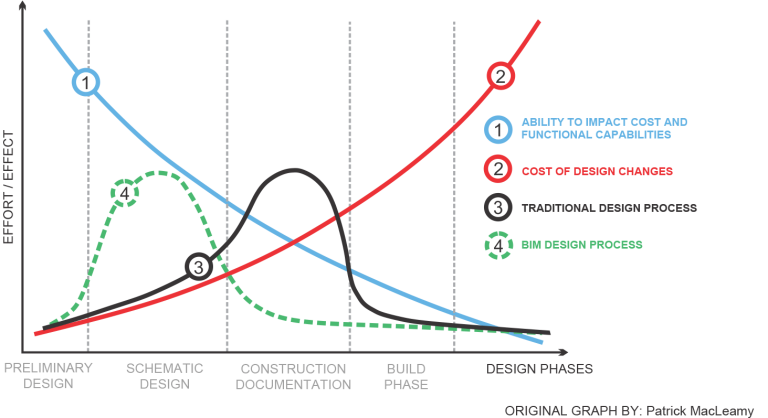
\includegraphics[width=0.5\textwidth]{figures/BIM grafiek.png}
    \caption{Evolution of \ac{lod} during the life-cycle of a building.}
    \label{fig:bimGraph}
\end{figure}

As shown in figure~\ref{fig:bimGraph}, a standard BIM workflow goes through multiple fases each with there assosiated model and \ac{lod}. The \ac{lod} is a very important concept in the \ac{aec} industry, as it allows for a very efficient workflow. Approaching the modeling step from a top-down perspective, starting with rougher geometries descriving the rougher ideas of a concept model and evoluting to a more refined model for the construction fase. As last and longest standing model, can a higher \ac{lod} be used to describe suttle changes in the evolution of a building.

This amount of data, both accounting for the \\
-> Some data BB models

\subsection{\acs{ldbim}}
% -> ! Focus on geometry

% -> What is \ac{ldbim}?

% -> Why the need / What are the advantages of \ac{ldbim}?

% -> Context od enrichment and complexity

-> Own definition of \ac{ldbim}

The interconnectivity of semantics can also be applied to geometry descriptions. Which could allow the co-existance of multiple \ac{lod}'s in a single model. Besides storing the evolution of an single element's geometry, it allows the linking of the different \ac{lod}'s to each other. In contrary to a standard \ac{bim} models, as explained in \ref{subsec:bimGeometry}.

\subsection{Computing power dilemma}
The enrichment of the \ac{ldbim}-graph also comes with a cost. The amount of data that needs to be stored and processed is much larger than a standard \ac{bim} model. Viewers greatly suffer from enrichment as most standard applications require the full model to be loaded in memory.

-> What is the hardware problem?

-> Why is it that important for the \ac{aec} industry?

\section{Research questions}

-> Why the need for this thesis? (why a \ac{ldbim} viewer?)

-> What is the possible solution? (Culling algorithms)

-> Why the need for research questions?
(culling algorithms are not new, always progress, see later)

\subsection[Can \acs{ldbim} be culled?]{To which extent can \acs{ldbim} geometry be culled\\
    to be streamed to lightweight viewers?}
-> What can be culled exactly?

-> What needs to be streamed?

-> What is the impact of culling on the viewing experience?

\subsection[Can existing semantic be used?]{Can existing semantic and ontologies be used to\\
    feed possible culling algorithms?}
-> What are ontologies?

-> Can GIS ontologies be used too?

-> What are the advantages of using ontologies?

\section{Research objectives}
\subsection[Advantages of LDBIM]{Bring forward the advantages of \acs{ldbim} for visualization of big 3D models}
-> Showcase that existing models are already mature enough for these usecases.

->
\subsection[Showcase the fisability]{Showcase the fisability of \acs{ldbim} for visualization of big 3D models}
->